\section{Symbolic Execution}
\label{sec:symExec}

%Introduce symbolic execution
Symbolic execution~\cite{Cadar-EXE} is a well-known technique for automatically detecting bugs and security vulnerabilities in a program. Among various challenges facing symbolic execution, handling symbolic memory addresses (addresses derived from user-input) is an important one. There are two primary approaches for handling symbolic memory. Previous symbolic executors for executables~\cite{Song-Bitblaze, Chipounov-S2E} make simplifying and unsound assumptions by concretizing the symbolic memory reference to a fixed memory location. On the other hand, popular source-level tools like EXE~\cite{Cadar-EXE} and KLEE~\cite{Cadar-KLEE} employ logical constraint solvers to reason about possible locations referenced by a symbolic memory operation. Even though the expressions involving symbolic memory become more sophisticated, these tools outperform the former approaches in terms of path exploration and bug detection.

%The main principle behind this technique is to represent the program inputs with symbolic values instead of concrete input values, and execute the program by manipulating symbolic program expressions. 
%The symbolic expressions along a program path are maintained as a set of constraints. At each potentially vulnerable program point, constraint solvers are employed to check if an input value exists that can trigger an error. The symbolic memory access arises whenever the address in a memory reference instruction is an expression derived from the user input.

\begin{figure}[t]
{
%\vspace{-0.2in}
%\begin{minipage}[t]{0.68\linewidth}
\begin{minipage}{0.68\linewidth}
\centering
{
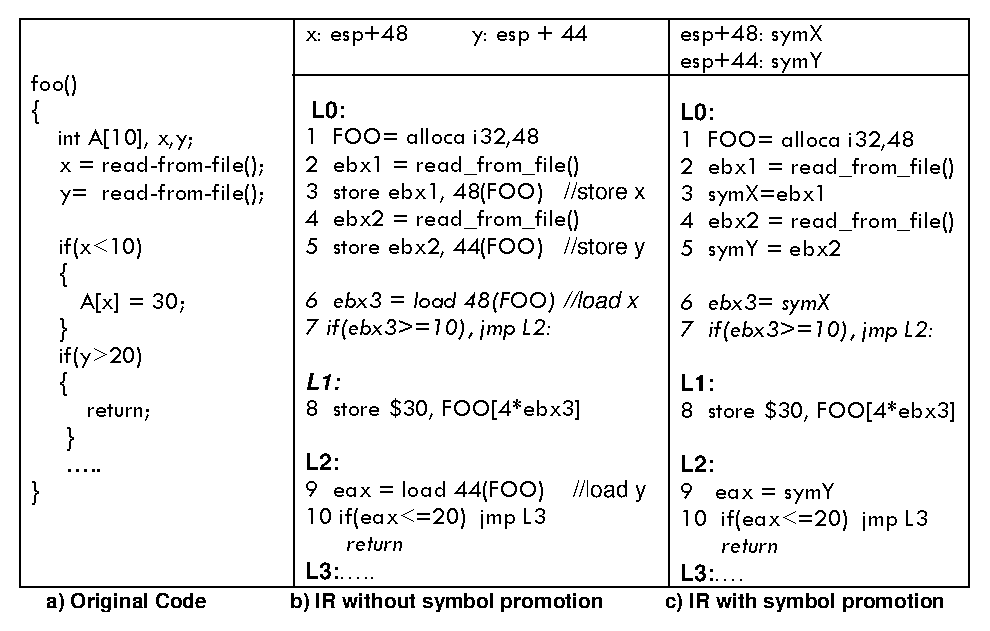
\includegraphics[width=\linewidth]{figures/EPS/symExecution.eps}
\vspace{-2ex}
\caption{\textit{A small source code example}}
\label{fig:symExecSourceCodeEx}
}
\end{minipage}
\hfill
\begin{minipage}{0.3\linewidth}
\centering
{
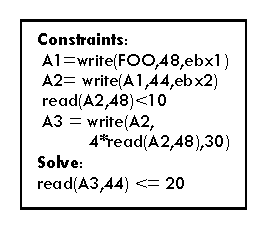
\includegraphics[width=\linewidth]{figures/EPS/symExecConstraints.eps}
\vspace{-2ex}
\caption{\textit{Constraints for Fig~\ref{fig:symExecSourceCodeEx}(b)}}
\label{fig:symExecSourceConstraints}
}
\end{minipage}
\vspace{-2ex}
}
\end{figure}


%Introduce symbolic memory
%, in case any path condition is dependent on an index.  
%One approach is to concretize the symbolic address while the other approach is to simulate a fully symbolic memory.
%Even though these assumptions greatly simplify the subsequent symbolic formulas, it might result in symbolic execution tool to miss some paths.

%\begin{figure}[t]
{
%\vspace{-0.2in}
\centering
%\psfig{figure=figures/plots/runtimeFinal.eps,width=5.5in} }
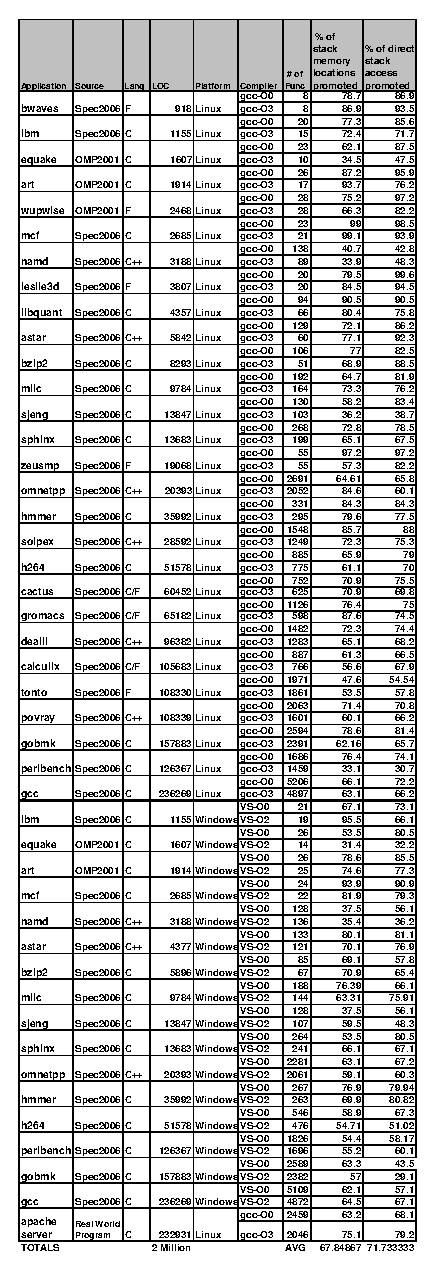
\includegraphics [width=0.7\linewidth] {figures/EPS/appTablenew2.eps} 
%\vspace{-3ex}
\caption { \textit{Benchmarks Table}}
\label{fig:appTable}
}
\vspace{-2ex}
\end{figure}

%Various symbolic execution systems like BitBlaze~\cite{Song-Bitblaze, Chipounov-S2E} make unsound assumptions by concretizing the symbolic memory reference to a fixed memory location. These assumptions greatly simplify the subsequent symbolic formulas obtained while exploring the program paths. However, constraining the memory reference to a fixed location might result in symbolic execution tool to miss some paths, in case any path condition is dependent on an index.  

%Various popular symbolic execution tools like EXE~\cite{Cadar-EXE}, KLEE~\cite{Cadar-KLEE} are based on the latter approach. These tools employ logical constraint solvers to reason about the possible locations referenced by a symbolic memory operation. Even though the program expressions involving symbolic memory are more sophisticated, these tools have been shown to outperform the former approaches in terms of path exploration and bug detection in the programs.

%Why is is more important at binary level
The presence of a physical stack and the lack of symbols in an executable pose a difficult challenge in efficiently extending the logical solver based approach for representing symbolic memory in executables. The most straightforward representation of the memory would be a flat byte array. Unfortunately, the  constraint solvers employed in existing source-level symbolic execution tools would almost never be able to solve the resulting constraints~\cite{Cadar-KLEE}. 

%Some idea about how symbolic promotion solves this challenge
The segmented memory representation in our framework, obtained by abstract stack and symbol promotion, drastically improves the efficiency of such constraint solvers by enabling them to only consider the constraints related to the segments referenced by the current memory address expression and ignore the remaining segments.
% ignore the constraints related to all other segments, thereby, drastically improving their efficiency. 
%In the following discussion, we use the standard notation for representing memory references in case of symbolic execution, where the operation \emph{read(A,i)} returns the value at index i in a  memory array A and \emph{write(A,j,v)} returns a new array with same value as A at all indices except i, where it has value v. Various source level symbolic execution tools map every memory object in the program code to a distinct array. This representation dramatically improves performance since it lets the constraint solvers ignore all arrays not referenced by a given expression. 

Fig~\ref{fig:symExecSourceCodeEx} illustrates this case. Fig~\ref{fig:symExecSourceCodeEx}(a) contains a symbolic memory store to array A. Fig~\ref{fig:symExecSourceCodeEx}(b) and Fig~\ref{fig:symExecSourceCodeEx}(c) show the pseudo IR obtained from an executable corresponding to Fig~\ref{fig:symExecSourceCodeEx}(a), without and with the application of symbol promotion. Fig~\ref{fig:symExecSourceConstraints} shows the constraints and query generated at Line 10 while symbolically executing the path L0$\rightarrow$L1$\rightarrow$L2 in Fig~\ref{fig:symExecSourceCodeEx}(b). Here, \emph{read(A,i)} returns the value at index i in array A and \emph{write(A,j,v)} returns a new array with same value as A at all indices except j, where it has value v.
%\begin{figure}[h]
%\vspace{-3ex}
%\centering
%{
%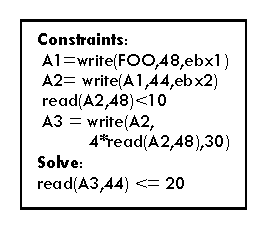
\includegraphics[width=0.3\linewidth]{figures/EPS/symExecConstraints.eps}
%}
%\end{figure}
%\vspace{-3ex}

However, in Fig~\ref{fig:symExecSourceCodeEx}(c), symbol promotion has segmented the array FOO in different segments and references to variables x and y do not refer the segment FOO. Hence, the solver only needs to solve the following simplified query:

{\begin{scriptsize}
\vspace{-2ex}
\begin{equation}
{\scriptsize 
Solve: symY \leq 20
}
\end{equation} 
%\vspace{-2ex}
\end{scriptsize}}
}
%without any constraints
This example only shows the simplification of constraints with symbol promotion. The presence of an abstract stack also results in a similar simplification of constraints by segmenting the memory space within each procedure.
